



%% ****** Start of file apstemplate.tex ****** %
%%
%%
%%   This file is part of the APS files in the REVTeX 4 distribution.
%%   Version 4.1r of REVTeX, August 2010
%%
%%
%%   Copyright (c) 2001, 2009, 2010 The American Physical Society.
%%
%%   See the REVTeX 4 README file for restrictions and more information.
%%
%
% This is a template for producing manuscripts for use with REVTEX 4.0
% Copy this file to another name and then work on that file.
% That way, you always have this original template file to use.
%
% Group addresses by affiliation; use superscriptaddress for long
% author lists, or if there are many overlapping affiliations.
% For Phys. Rev. appearance, change preprint to twocolumn.
% Choose pra, prb, prc, prd, pre, prl, prstab, prstper, or rmp for journal
%  Add 'draft' option to mark overfull boxes with black boxes
%  Add 'showpacs' option to make PACS codes appear
%  Add 'showkeys' option to make keywords appear
%\documentclass[aps,prb,preprint,superscriptaddress,showkeys,endfloats]{revtex4-1}
%\documentclass[aps,prb,preprint,superscriptaddress,showkeys]{revtex4-1}
\documentclass[aps,pre,reprint,superscriptaddress,showkeys]{revtex4-1}
%\documentclass[ aip, jmp, bmf, sd, rsi, amsmath,amssymb, preprint, reprint, author-year, author-numerical,Conference Proceedings]{revtex4-1}
\usepackage{amsmath}
\usepackage{color}
\usepackage{graphicx}
\usepackage{dcolumn}
\usepackage{verbatim}
\usepackage{epstopdf}
\usepackage{inputenc}
\usepackage{amssymb}

\newcolumntype{d}{D{.}{.}{-1}}





\begin{document}





\title{First principles calculation of the configurational energy density of states for LLTO with new Wang and Landau algorithm variant }

\author{Jason D. Howard}
\affiliation{Materials Science Division, Argonne National Lab, Lemont, IL, 60439, USA}
\email{jdhoward@anl.gov}
\date{\today}


\begin{abstract}
In this work  a variant of the Wang and Landau algorithm   for calculation of  the configurational energy density of states is proposed. The algorithm was developed for the purpose of   using first principles simulations, such as density functional theory, to calculate the partition function of disordered sublattices in crystal materials. The expensive calculations of first principles methods make a parallel algorithm necessary for a practical computation of the configurational energy density of states within a supercell approximation of a solid state material.  The algorithm developed in this work is tested with the 2d Ising model to bench mark the algorithm and to help provide insight for implementation to a materials science application. Tests with the 2d Ising model revealed that the algorithm has good performance compared to the original Wang and Landau algorithm and has similar behavior to the N-fold 1/t algorithm. The algorithm was then applied to the lithium and lanthanum sublattice of the solid state lithium ion conductor Li$_{0.5}$La$_{0.5}$TiO$_{3}$. This was done to help understand the disordered nature of the lithium and lanthanum. The results find, overall, that the algorithm performs very well for the 2d Ising model and that the results for Li$_{0.5}$La$_{0.5}$TiO$_{3}$ are consistent with experiment while providing additional insight into the lithium and lanthanum ordering in the material. The primary result is that configurations with lithium and lanthanum more mixed between layers tend to be higher in energy. 
\end{abstract}
\maketitle
\section{Introduction}
For crystalline  materials  with disordered sublattices such as the lithium ion solid state electrolyte LLTO it is desirable to calculate from first principles methods(such as density functional theory\cite{kohn:1965}) the configurational energy density states $G(E_j)$, which will simply be referred to as the density of states. Here the  density of states refers to the energies of the distinct lattice configurations. With the  density of states the partition function,
\begin{equation}
\begin{split}
Z = \sum_{i}^{\Omega}e^{\frac{-e_i}{k_B T} }= \sum_{j}^{\Pi}G(E_j)e^{\frac{-E_j}{k_BT}} \;,
\end{split}
\label{partition}
\end{equation}
can be  determined and from it many important thermodynamic properties such as the free energy, entropy, specific heat, and ensemble averages calculated. In Eq. (\ref{partition}), $\Omega$ corresponds to the total number of possible  configurations($\Sigma_i$) and energies($e_i$) referred to by the set $\{\Sigma_i,e_i\}_\Omega$, $\Pi$ is the number of possible distinct energies $E_j$ that appear in $\{\Sigma_i,e_i\}_\Omega$, $k_B$ is Boltzmann's constant, and $T$ is the temperature. If $\Omega$ is small enough one of the simplest ways to estimate $G_r(E_j)$ could be direct random sampling of the configuration space\cite{partition}, which does have the advantage of being compeletly parrallel. For most problems $\Omega$ will be too large to allow direct random sampling of the configuration space to be practical, making an importance sampling algorithm necessary. A very well known importance sampling method to solve this problem could be temperature dependent simulations involving the Metropolis algorithm and sampling with probability proportional  to $exp(\frac{-e_i}{k_B T})$ 
along with histogram re-weighting techniques\cite{metropolis_equation_1953,histogram_reweighting, landau_MC_simulations}. Another more advanced method is the multi-canonical method proposed by Berg et al. \cite{Multi_Canonical,multi_canonical_two}. A variant of multicanonical sampling that samples the density of states directly known as entropic sampling developed by Lee \cite{Entropic_Sampling} could also be used. 
The multicanonical method requires a careful choice of simulation paramaters while the entropic sampling requires a good estimate of the density of states to be effective.  Another algorithm called the  Wang and Landau algorithm \cite{WL_phys_rev_lett,Wang_Landau_phys_rev_E} has been developed which is temperature independent, is based on a random walk in energy space with probability inversely proportional to the current estimate of the  density of states, and builds up the  density of states as the algorithm progresses.  An issue with these algorithms(if using a single walker) in use with first principles methods such as density functional theory is the large number of iterations needed, which would require a prohibitively long wall time at the current performance power of computers.  In this paper an algorithm is proposed that combines the use of random sets along with the importance sampling method of the Wang and Landau algorithm. The algorithm also used the principle of the Wang and Landau algorithm to build up an estimate of the  density of states as the algorithm progresses.  The proposed algorithm is meant to work towards the goal of a highly parallel importance sampling algorithm that directly calculates the  density of states, meshes well with mid level high performance computing architectures(such as Argonne's BEBOP), and has a minimum of paramaters for implementation. The algorithm developed in this work is referred to as the B$_{L}$ENDER (B$_{L}$end Each New Density Each Round) algorithm. 

    The Wang and Landau method does have parallel versions, including  restricting random walkers to specific energy ranges, allowing the walkers to explore the entire space while periodically communicating with each other, and methods based on a replica exchange frame work \cite{MP_Wang_Landau,P_imp_Wang_Landau, Hframe_Wang_Landau, Scalable_replica_exchange}.  The B$_{L}$ENDER algorithm is characterized by allowing the walkers to explore the entire energy range and communication with each other through an update to the density of states at each iteration.  In principle many of the different forms of  Wang and Landau sampling currently used are based around the concept of sampling until a flat histogram of the visited energies is reached followed by a reduction in a modification factor to the density of states and that the calculated density of states  is multiplied by this factor every time an energy level  is visited.  One issue with these types of Wang and Landau simulations is that, being based on a flat histogram of the visited energies, the energy range must be specified \textit{apriori}. Another issue is that the original Wang and Landau formulation for the reduction in the modification factor to the  density of states has been shown be non-convergent\cite{Non_convergent_WL,Non_convergent_WL_2,non_convergence_multiple_random_walkers,Optimal_modification}.   There have been advancements made in understanding how to reduce the modification factor by Belardinelli et al. \cite{saturation} whom developed the 1/t algorithm which is proven to be convergent, this result was verified by the work of Zhou et al. \cite{Optimal_modification}. An issue with the 1/t algorithm as presented by Belardinelli et al. is that it requires a non-trivial preconditioning using what is referred to as the N-fold way. The N-fold way requires a careful analysis of the  method to perturb the systems affect on the energy which for local models like the Ising model is possible but for first principles simulation this is not feasible. The novel aspects of the B$_{L}$ENDER algorithm include, a continuous adaptation of the modification factor to the  density of states using the current sum of the density of states as a regulator, using the number of configurations as a parameter in the modification factor, and using a histogram of the currently visited energies as a parameter in the modification factor.  The algorithm in this work is believed to be convergent based on its comparison with the 1/t algorithm and from mathematical analysis within an adiabatic assumption. The algorithm is also natural to parallelize as it is based on a set of random walkers. The algorithm was developed for ease of use in the application to disordered sublattices of crystal systems. 

   In this work the formulated algorithm is benched marked with the 2d Ising model as a standard means of testing  performance.  The tests allow for a comparison to exact results and to previous benchmarks of other algorithms. The tests with the 2d Ising model also allow for insight in how to implement the algorithm to a materials science problem. The main goal in this work  was to calculate with first principles methods the  density of states of the lithium ion conductor Li$_{0.5}$La$_{0.5}$TiO$_3$. There  have been  reports of the Wang and Landau algorithm used with linear scaling density functional theory methods to calculate magnetic properties of materials and order to disorder properties of alloys\cite{Eisenbach, FP_Wang_Landau_CuZn}. There has also been a report of first principles calculations with replica exchange canonical Metropolis sampling for investigating ion disorder in solids by Kasamatsu et al. \cite{ion_disorder_replica}.  Li$_{0.5}$La$_{0.5}$TiO$_3$ is part of a family of possible stoichiometries Li$_{3x}$La$_{2/3 -x}$TiO$_3$ of interest as solid state lithium ion conductors\cite{domainboundaries,P4mmmstrucuture,imaginary_phonons,GENG2009555,peculiarities,LLTOreview,Li_La_ordering_computational}. For all of the possible stoichiometries there is a tendency towards ordering of the lithium and lanthanum into lithium rich layers and lanthanum rich layers.  The primary calculation of this work is that of the temperature dependent order parameter related to the lanthanum rich layer in Li$_{0.5}$La$_{0.5}$TiO$_3$. This calculation both serves to benchmark the application of the algorithm to a materials science problem with experimental knowns and to provide further insight into the physics of the material. 
   
   The rest of the article is organized as follows; section \ref{sec1} explains the B$_{L}$ENDER algorithm, section \ref{sec2} covers the testing of the algorithm with the 2d Ising model including comparison with the original Wang and Landau algorithm and N-fold 1/t algorithm, section \ref{sec3} covers an adiabatic analysis of the alorithms convergence and the time dependence of the modification factor, section \ref{sec4} covers the application of the algorithm to LLTO along with the computational details of the first principles methods, and section \ref{sec5} is the conclusions. 
   
   In this work the software package XMGRACE\cite{XMGRACE} was used in the generation of plots and VESTA\cite{Vesta}  for the generation of structural images of LLTO.

\section{Algorithm}
\label{sec1}
The B$_{L}$ENDER algorithm proposed in this work  is given as follows for $\mathcal{S}$ random walkers. It is noted that the following algorithm is in terms of producing a relative density of states $G_{r}(E_j)^I$, where $I$ is the iteration number. 

\begin{equation}
\begin{split}
&1.\hspace{0.125cm} G_{r}(E_j)^I ,\hspace{0.15cm}  \{\Sigma_{s},e_s\}_{\mathcal{S}}^I\\
&2. \hspace{0.125cm}\{\Sigma_{s},e_s\}_{\mathcal{S}}^I \rightarrow  \{\Sigma_{s}^{'},e_s^{'}\}_{\mathcal{S}}^I\\
&3. \hspace{0.125cm} \Sigma_{s}^{'I}, e_s^{'I} \rightarrow \Sigma_{s}^{I+1},e_s^{I+1}   \hspace{0.125cm} P = \hspace{0.075cm} min [1, G_r(e_s)^{I}/G_r(e_s^{'})^{I}]\\
& \hspace{0.125cm}else  \hspace{0.15cm} \Sigma_{s}^I, e_s^I \rightarrow \Sigma_{s}^{I+1}, e_s^{I+1}\\
&4. \hspace{0.125cm} G_{r}(E_j)^{I+1} =  \\
& G_{r}(E_j)^{I} + \frac{C_o \mathcal{H}^I }{ (A^{I})^{\frac{1}{N} } }G_{r}(E_j)^{I} = \\
& G_{r}(E_j)^{I}( 1 +  \frac{C_o \mathcal{H}^I }{ (A^{I})^{\frac{1}{N} } } )\\
\end{split}
\label{blender}
\end{equation}
%Where  $G_{r}(E_j)^0 \equiv [1 +  \frac{C_o}{S}\mathcal{H}(E_j,\{e_s\}_{\mathcal{S}}^0)]$ 
Where  $\mathcal{H}^I \equiv \mathcal{H}(E_j,\{e_s\}_{\mathcal{S}}^I)$, that being an  histogram function that counts the number of the currently vistied  energies $E_j$ in the set $\{e_s\}_{\mathcal{S}^I}$. The ``instantaneous'' histogram $\mathcal{H}^I$ is related to the total histogram of visited energies $H^I(E_j)$ by $H^I(E_j) = \sum_{i=0}^{I}\mathcal{H}^i$. The value $A^I \equiv \sum_jG_r(E_j)^I$.  In this work $\{\Sigma_{s},e_s\}_{\mathcal{S}}^0$  is a randomly drawn set of $\mathcal{S}$ walkers from the configuration space $\{ \Sigma_i, e_i \}_\Omega $. Also in this work the initial guess of the density of states was set to $G_{r}(E_j)^0 = 1 +  \frac{C_o}{S}\mathcal{H}^0$, but in principle there could be other ways to intitialize the initial guess to the density of states. In the second step  a random change is applied to each element of the sampled set $\{\Sigma_{s},e_s\}_{\mathcal{S}}^I$ to produced a ``perturbed" set $ \{\Sigma_{s}^{'},e_s^{'}\}_{\mathcal{S}}^I$ , for the Ising model this could be randomly flipping a spin.  In the third step a random number is drawn between zero and one for every sampled configuration, if this number is less then the ratio of the current density of states of the unperturbed to perturbed energies $G_{r}(e_s)^{I}/G_{r}(e_s^{'})^{I}$ then the perturbed configuration and energy  $\Sigma_{s}^{'I},e_s^{'I}$  goes to $\Sigma_{s}^{I+1},e_s^{I+1}$,  else the unperturbed configuration and energy $\Sigma_{s}^{I},e_s^I$  goes to $\Sigma_{s}^{I+1},e_s^{I+1}$. This step (third) is derived from the Wang and Landau method of sampling with probability inversely proportional to the density of states.  In the fourth step a histogram of the updated $\{ e_s \}^{I+1}_{\mathcal{S}}$ energies is made and added (blended) into the current density of states $G_{r}(E_j)^I$   by multiplying  by a constant $C_{o}$(which affects the convergence properties) and   $G_{r}(E_j)^{I}$ divided by the sum of the density of states to the $1/N$ power. The $1/N$ power is introduced as tuning parameter to affect the convergence properties and was discovered through empirical testing with the 2d Ising model.  The fourth step is also shown in terms of multiplication which is discussed later. In this work it was found  $C_{o}=\Omega^{\frac{1}{N}}$ was computationally efficient. After the algorithm is deemed to be complete it is necessary to renormalize the iterated relative density of states $G_{r}(E_j)^f$ at the final iteration $I=f$ as follows, 
\begin{equation}
\begin{split}
&1. \hspace{0.125cm} A^f = \sum_jG_{r}(E_j)^f\\
&2. \hspace{0.125cm} G_{calc}(E_j) = G_{r}(E_j)^f \frac{\Omega}{A^f} \;,
\end{split}
\label{renormalize}
\end{equation}
to produce the properly normalized estimated value of $G(E_j)$. In principle, $G_{r}(E_j)$ can also be renormalized based on information of the number of configurations in a given bin. For example if the ground state is known to have a given degeneracy then the entire density of states can be normalized such that the ground state bin has the correct degeneracy. 

 


An important discussion point of this algorithm (Eq. \ref{blender}) is the update of the relative density of states(step four) being presented as addition and multiplication.
 In  typical Wang and Landau sampling the update of the density of states is preformed by multiplication of the density of states by a factor greater than one every time an energy level is visited combined with a periodic reduction of the multiplication factor towards one when a histogram of visited energies reaches a predetermined flatness criteria, the histogram of the visited energies is then reset to zero. In the multiplication form of step four of this algorithm (Eq. \ref{blender}) it is seen that the dependence on one over the sum of the density of states serves to naturally reduce the multiplication factor towards one as the simulation progresses. The multiplication form is also useful when $\Omega$ is large and the sum of the density of states is larger than a typical floating point number. In this case the log of the density of states can be stored and the update performed through addition of logs. Taking $G_{r}^M \equiv  max[G_{r}(E_j)]$ the log of $A^{I}$ can be written as, 
\begin{equation}
\begin{split}
& \log[A^{I}] = \log[G_{r}^M \frac{A^{I}}{G_{r}^M}]=\\
&\log[G_{r}^M] + \log[\sum_j e^{\ln[G_{r}(E_j)] - \ln[G_{r}^M]} ] \;.
\end{split}
\label{Hls}
\end{equation} 
With $G_r^{LS}$ from Eq. \ref{Hls} the $\log$ update form of step four of the algorithm (Eq. \ref{blender}) can be written as the following, 
\begin{equation}
\begin{split}
& \log[ G_{r}(E_j)^{I}( 1 +  \frac{C_o \mathcal{H}^I }{ (A^{I})^{\frac{1}{N} } } ) ]=\\
& \log[ G_{r}(E_j)^{I} ] + \log[1 +   \mathcal{H}^Ie^{\ln[C_o]-\frac{1}{N}\ln[A^{I}]}] \;.
\end{split}
\end{equation}
In this form  the algorithm can be implemented even when $\Omega$ is large. To implement the ratio of the density of states in step two of the algorithm, 
\begin{equation}
e^{\ln[G_{r}(e_s)^{I}] - \ln[G_{r}(e_s^{'})^{I}]} \;,
\end{equation}
can be used.

 

\section{Bench mark with 2d Ising model}
\label{sec2}

In this work the algorithm discussed is tested using the 2d square zero field  Ising model with lattice dimension of even number\cite{exact_statistical,Onsager,Ising} and periodic boundary conditions. The configurations $\Sigma_i$ and energies $e_i$ of the 2d Ising model are inherently defined by the lattice site spin variables $\sigma_{k,l}$ which take the values $\pm 1$ and coupling constant $J$. Explicitly the energy $e_i$ for a given configuration $\Sigma_i$ of a n$\times$n Ising lattice is given by, 
\begin{equation}
e_i = -J\sum_{k,l=1}^{n}\sigma_{k,l}^{i}(\sigma_{k+1,l}^{i} + \sigma_{k,l+1}^{i})\;.
\end{equation}

\subsection{Performance and properties of the B$_L$ENDER algorithm}
  The first test is the effectiveness of the algorithm in calculating the density of states of the 2d Ising model.  To test the accuracy of the simulations the results will be compared to the exact result solved by Beale \cite{Beale_2d_ising}. The accuracy of the simulation will be determined by the error defined as, 
\begin{equation}
\begin{split}
 &\mathcal{E}(I) \hspace{0.1cm}= \hspace{0.1cm}< |\epsilon(E_j,I)| >_j\\
& = \hspace{0.1cm}  \frac{1}{\Pi} \sum_{j=1}^{\Pi}\frac{|\ln[G_{ex}(E_j)]- \ln[G_{calc}(E_j,I)]|}{|\ln[G_{ex}(E_j)]|}\; 
 \end{split}. 
 \label{avg_error}
\end{equation}

Where $G_{ex}(E_j)$ is the exact density of states, $G_{calc}(E_j,I)$ is the calculated density of states from Eq. \ref{renormalize}  at iteration number $I$ , and $|\epsilon(E_j,I)|$ is the absolute value of the fractional error for a specific energy level.  The perturbed configurations in this work were generated by randomly flipping one spin on the Ising lattice

The first test of the algorithm is with the 32$\times$32 Ising model. In a materials science problem with first principles calculations the system size is not expected to be anywhere near the size of the  32$\times$32 Ising model so these results are included to show the algorithm has potential for larger system sizes. While the ideal value of $N$ is not known prior to the calculation it was found in this work that a value of $1/N=$ 0.1 was computationally efficient for the 32$\times$32 Ising model. In Fig. \ref{thirtytwo_Stest}(a) the value of the average error calculated with Eq. \ref{avg_error} is shown up to 1e7 iterations for $\mathcal{S}=$ 1 , 10, 100, 1000, and 1e4. The data in Fig. \ref{thirtytwo_Stest}(a) is averaged over 36 individual simulations for each value of $\mathcal{S}$. At $I=$ 1e7 The results show linear scaling from $\mathcal{S}=$ 1 to $\mathcal{S}=$ 10 and then another order of magnitude improvement from $\mathcal{S}=$ 10 to $\mathcal{S}=$ 1000, and at $\mathcal{S}=$ 1e4 there is marginal improvement at $I=1e7$ but worse performance for $I<1e6$.  The periodic fluctuations in the average error are also noted in going to larger $\mathcal{S}$, these flucations are due to the calculated density of states(renormalized) oscillating about the exact solution and that for larger $\mathcal{S}$  these flucations are more in sync with each from one calculation to the next leading to a smooth average. For large $\mathcal{S}$ movies of convergence show that the wings of the density of states get more stretched before the walkers have completely scanned the energy range which leads to calculated soluion experiencing large oscilations about the exact solutions on the wings. A further discussion of these flucations along with movies of convergence can be found in the supplemental materials.  In Fig. \ref{thirtytwo_Stest}(b) are  the results for the average error of 36 independent simulations of a 10$\times$10 Ising model for the different number walkers $\mathcal{S}=$ 1 , 10, 100, 1000, and 1e4, and  with $N=$ 1. The results show that the scaling is quite good as the number of walkers increases. This result is encouraging because the number of configurations that would be typical for a supercell approximation in a density functional theory calculation is not expected to exceed the large number of $\approx 10^{30}$ configurations in the 10$\times$10 Ising model.  Although in the work of  Kahn et al. \cite{FP_Wang_Landau_CuZn} they did tackel a configuration space of size of $ 10^{74}$ using linear scaling density functional theory for a 250 atom supercell. Typical density functional theory calculations scale roughly as the cube of the number of atoms, so their calculation was only feasible using the linear scaling methods.   
\begin{figure}[h!]
(a)\\
\includegraphics[width=8.6cm]{fig1a.eps}\\
(b)\\
\includegraphics[width=8.6cm]{fig1b.eps}
\caption{(color online) Average error from 36 simulations calculated with Eq. \ref{avg_error} with $\mathcal{S}=$ 1, 10, 100, 1000, and 1e4 for  (a) the 32$\times$32 Ising model with $1/N=$ 0.1, (b) the 10$\times$10 Ising model with $1/N =$ 1. \label{thirtytwo_Stest} }
\end{figure}

Another aspect of the algorithm to consider is the dependence on the value of $N$ and of $C_{o}$. In Fig. \ref{N_dependence}(a) and (b) the dependence on $N$ is shown for  the 32$\times$32  and  10$\times$10 Ising models, simulated to $I=$ 1e7 and $I=$ 1e6 respectively for $\mathcal{S}=$ 100  (a) and $\mathcal{S}=$ 10  (b). The results in Fig. \ref{N_dependence}(a) and (b) were averaged over 36 independent simulations. The results in Fig. \ref{N_dependence}(a) show that for the larger 32$\times$32 model with $\mathcal{S}=$ 100 the dependence on $N$ is more pronounced and that the optimal value of $1/N$ is lower than for the  32$\times$32 model with $\mathcal{S}=$ 10 and the  smaller 10$\times$10 model for both $\mathcal{S}=$ 10 and $\mathcal{S}=$ 100. The more pronounced convergence dependence on $N$ for the larger 32$\times$32 model at larger $\mathcal{S}$ does pose a problem if one was to implement the the algorithm for a new system where the density of states is not known beforehand because there is no current evidence to predict what the optimal parameter would be.  The tests with the 10$\times$10 model suggest that for a smaller system size that the convergence dependence on $N$ is less pronounced and that $N=$ 1 is sufficient. The results presented here suggest that if one was to use the algorithm for a larger system size some method of predicting the optimal value of $N$ would be required. These tests have used a value of $C_{o}=\Omega^{1/N}$, this value was based on tests showing this to be a computationally efficient choice that can be predicted based on knowledge of the system. In Fig. \ref{optimalCo}(a) and (b)  is shown the error for the 32$\times$32 and 10$\times$10   Ising model vs $C_{o}/\Omega^{1/N}$ with, $1/N=$ 0.1 and $1/N=$ 1 respectively, $I=$ 1e7 and $I=$ 1e6 respectively, and with $\mathcal{S}=$ 100  (a) and $\mathcal{S}=$ 10  (b). The results in Fig. \ref{optimalCo}(a) and (b) were averaged over 36 independent runs. The results in Fig. \ref{optimalCo}(a) and (b)  show that the errors are relatively insensitive to the value of $C_{o}$ within several orders of magnitude of $\Omega^{1/N}$ and that the main feature is a sudden increase in error going below some lower bound of $C_{o}$ and a plateau of the error for $C_{o}$ above this lower bound. 

\begin{figure}[h!]
(a)\\
\includegraphics[width=8.5cm]{fig2a.eps}\\
(b)\\
\includegraphics[width=8.5cm]{fig2b.eps}\\

\caption{(color online) Average error calculated from Eq. \ref{avg_error} from 36 simulations for (a) $\mathcal{S}=$ 10 and (b) $\mathcal{S}=$ 100   vs the value of $1/N$ for the 32$\times$32 (red circles) and 10$\times$10 (blue squares) Ising models simulated to 1e7 and 1e6 iterations respectively.  Errorbars show the standard deviation of the mean. \label{N_dependence}}
\end{figure}

\begin{figure}[h!]
(a)\\
\includegraphics[width=8.6cm]{fig3a.eps}\\
(b)\\
\includegraphics[width=8.6cm]{fig3b.eps}\\
\caption{(color online) Average error from 36 simulations calculated from Eq. \ref{avg_error} for the 10$\times$10(black circles) and 32$\times$32(red squares) Ising model simulated to 1e6 and 1e7 iterations and  with $1/N=1$ and $1/N=$ 0.1 respectively for (a)  $\mathcal{S}=$ 10 and (b) $\mathcal{S}=$ 100 vs the value of $C_{o}/\Omega^{1/N}$. Error bars show the standard deviation of the mean.  \label{optimalCo}}
\end{figure}

\subsection{Comparison with original Wang and Landau algorithm}
In Wang and Landau's original work they simulated  32$\times$32 and 50$\times$50 2d Ising models for comparison to the exact density of states. The comparison in this section will use the 32$\times$32 Ising model. To implement the original Wang and Landau algorithm the same parameters from their original paper will be used\cite{WL_phys_rev_lett}. First referring to the the historgram $H(E_j)\equiv \sum_{i=0}^{I}\mathcal{H}^I$, that is the histogram of the visited(accepted) energies during the simulation. Then defining the modification factor $f$ such that everytime a energy level is visited(accepted) then $G_r(E_j)^{I+1} = G_r(E_j)^{I}f$. In Wang and Landau's original work they used a flatness criteria of $80\%$ and a reduction schedule of $f^{I+1}= \sqrt{f^{I}}$. The flatness criteria was described such that all energies $E_j$ had been visited and that  $min[H(E_j)]/avg[H(E_j)] > 0.8$. When the flatness criteria is meet the reduction schedule $f^{I+1}= \sqrt{f^{I}}$ is then implemented. The value of $f^0 = e^1$ was used. Initial configurations were generated randomly and $G_r(E_j)^0$ was set to 1 when implementing the original Wang and Landau algorithm.  In the this manner the B$_L$ENDER algorithm with $1/N = 0.1$ and $\mathcal{S}=1$ was compared to the perfomance of the original Wang and Landau algorithm. The results are shown in Fig. \ref{compare_blender_wl}(a), which are averaged over 36 independant simulations. The comparison shows a striking difference in the error,  the B$_L$ENDER algorithm  tends to decrease over the entire time span while the original Wang and Landau implementation  rises to a large peak early in the simulation then abrutly drops. At large number of iterations the error is nearly the same for both. To compare potential parrallel performance of the orginal Wang and Landau algorithm in a scheme similar to the B$_L$ENDER algorithm the update,
\begin{equation}
G_r(E_j)^{I+1} = G_r(E_j)^{I}f^{\mathcal{H}^I}\;,
\label{parallelscheme}
\end{equation}
is adopted. Where $\{e_s\}^{I+1}_{\mathcal{S}}$ and $\mathcal{H}^I$ are generated and function the same was an in Eq. \ref{blender}. In this manner a simulation was carried out with 100 walkers ($\mathcal{S}=100$) for the Wang and Landau alogrithm, with the same flatness criteria and reduction schedule as above, and for the B$_L$ENDER algorithm to 1e7 iterations. The results are shown in Fig \ref{compare_blender_wl}(b), which are averaged over 36 independant simulations. The results show that both parallel implementations have siginificant improvement for equivalent number of iterations but that the original Wang and Landau still suffers the problem of rising to a large peak and then dropping suddenly. Both algorithms are shown to have similar errors at a large number of iterations until at some point the original Wang and Landau algorithm saturates and the B$_L$ENDER algorithm conintues to converge. 

  One aspect of the tests so far in this work is that they have used a system size only as large as the 32$\times$32 Ising model.  Which in terms of number of configurations is very large for system sizes possible with density functional theory simulations but is small compared to many statistical models commonly studied in phyiscs.  In fact Wang and Landau orginally tested there algorithm with the 256$\times$256 Ising model, although they did this by placing walkers in different energy windows which required either building the larger model from smaller Ising lattices were the energy was known are doing a preliminary energy scan.  In this work it was desriable to perform a benchmark with an entirely expoloratory calculation of large 256$\times$256 Ising system. So starting from randomly generated confgiruations with $\mathcal{S}=1000$ the B$_L$ENDER algorithm was compared to the orginal Wang and Landau algorithm. It was found that utilizing $1/N=0.01$ that it was possible to simulate this model quite efficiently with the B$_L$ENDER algorithm as compared to the orginal Wang and Landau using the same parameters as in this section. These results can be considered as a preliminary test of the B$_L$ENDER algorithm for large system size and are found in the supplemental materials, which includes movies of the convergence of the density of states and free energy. 
\begin{figure}[h!]
(a)\\
\includegraphics[width=8.6cm]{fig4a.eps}\\
(b)\\
\includegraphics[width=8.6cm]{fig4b.eps}\\
\caption{(color online) Average error from 36 simulations for the orginal Wang and Landau algorithm in red with circles and the B$_L$ENDER  algorithm in black with squares for (a) $\mathcal{S}=1$ simulated to 1e9 iterations and (b) $\mathcal{S}=100$ simulated to 1e7 iterations. \label{compare_blender_wl}}
\end{figure}

\subsection{Relationship of the B$_L$ENDER algorithm to the N-fold 1/t algorithm}
\label{test_wl}
In the introduction it was mentioned that an improvement to the update to the multiplication factor in the Wang and Landau method had been made by Belardinelli et al. \cite{saturation}, which was referred to as the 1/t algorithm. It was found in this work that for the $\mathcal{S}=$ 1, $N=$ 1, and $C_{o}=\Omega$ that the B$_L$ENDER algorithm had similar behavior to the results of Belardinelli et al.. To make the comparison we first consider the generic multiplication upate of the density of states
\begin{equation}
G_{r}(E_j)^{I+1} = G_{r}(E_j)^{I}f(I,E_j)\;.
\label{orignialform}
\end{equation}
For the B$_L$ENDER algorithm with $C_o = \Omega$ and $1/N=$ 1 $f(I,E_j)$ would take the form, 
\begin{equation}
f(I,E_j) = ( 1 +  \frac{\Omega \mathcal{H}^I }{ A^I } )\;.
\label{fequiv}
\end{equation}
For a single walker the value of $f(I,E_j)$ from Eq \ref{fequiv} will take the value of either $1$ or $(1+ \Omega/A^I)$. 
In the work by Belardinelli et al. They defined a value $F(t) = \ln[f(t)]$  and found an optimal form of $F(t) = \frac{c}{t^p}$, with $t$ being the effective Monte Carlo time defined for a single walker as,
\begin{equation}
t = \frac{I}{\Pi} \;.
\label{mcstep}
\end{equation} 
Where $\Pi$ is the number of energies $E_j$, which is ${n^2} -1$ for the $n\times n$  Ising model.   They found the optimal values to be $c=$ 1 and $p=$ 1. Also in their work they use a single walker and when they refer to $f(t)$ they are referring only to the value for the one bin being updated that iteration. To be effective though they found this algorithm required preconditioning with the original Wang and Landau algorithm. They also described a more complex variant of this algorithm called the N-fold 1/t  which incorporated the average life time of the initial configurations early in the simulation which then limited to the 1/t form.  In their work they used a 8$\times$8 Ising model, so to compare, calculations of the average of $F(t)=\ln(1+ \Omega/A^I)$  and the error defined by Eq. \ref{avg_error} from 36 simulations were done for the B$_L$ENDER algorithm.  The results for the average value of $F(t)$ are shown in  Fig. \ref{FtandA}(a) and the average error in Fig. \ref{FtandA}(b). In comparing the results to those taken from Fig. 5 of Belardinelli et al. \cite{saturation} shown in   Fig. \ref{FtandA} of this work, a striking similarity is seem in the behavior as compared to the N-fold 1/t algorithm. It is clear from this comparison that there is a mathematical relationship between these two algorithms although at the moment the exact nature of this relationship is unclear.  To further analyze the results of  Fig. \ref{FtandA}(a) it is noted that assuming $F(t) = \frac{m}{t^p}$  a linear fit of  $\log F(t)$ vs $\log(t)$ will predict the coefficients $c$ and $p$. Fitting the results from the B$_L$ENDER algorithm in Fig. \ref{FtandA}(a) in this manner gives $m=$ 1 and $p=$ 1. So the value of $p$ and $m$ is found to be in agreement with that of Belardinelli et al.. 
%These similarities with the N-fold 1/t algorithm, which is proven to be convergent, give further confidence in the B$_L$ENDER algorithm and suggest it is likely to be convergent as well. 


\begin{figure}
(a)\\
\includegraphics[width=8.6cm]{fig5a.eps}
\centerline{(b)}\\
\includegraphics[width=8.6cm]{fig5b.eps}
\caption{(color online) In black with squares (a) The average of $F(t)$ and (b) the average error defined by Eq. \ref{avg_error}  from 36 simulations of the 8$\times$8  Ising model with the B$_L$ENDER algorithm with $\mathcal{S}=$ 1, $N=$ 1, and $C_o = \Omega$. In red with circles (a) $F(t)$ results taken from the work of Belardinelli et al. \cite{saturation} (b) the error defined by Eq. \ref{avg_error} taken from the  work of Belardinelli et al.. Here $t = \frac{I}{63}$ or equivalently one Monte Carlo time step ($MC$) as defined by Eq. \ref{mcstep}.\label{FtandA} }
\end{figure}

\section{Adiabatic analysis of the algorithm}
\label{sec3}
To better understand the nature of the algorithm we will consider the adiabatic properties of the histogram $\mathcal{H}^I\equiv \mathcal{H}(E_j, \{e_s\}_\mathcal{S}^I)$. Considering that during a simulation the configurations are generated with probability proportional to $G(E_j)/\Omega$ and accepted inversely proportional to $G_{r}(E_j)^I/A^I$ the probability distribution, which we will write as $\Phi^I(E_j)$, of the $\mathcal{H}^I$ will be proportional to $[G(E_j)A^I]/[G_r^I(E_j)\Omega]$. For short we will write $G_r^I(E_j) \rightarrow G_r^I$, $G(E_j)\rightarrow G$, and $\Phi^I(E_j)\rightarrow \Phi^I$.  Considering that the sum over $\mathcal{H}^I$ is constrained to $\mathcal{S}$ if we normalize $\Phi^I$ to $\mathcal{S}$ we get
\begin{equation}
\Phi^I = \mathcal{S}(\sum_{j}\frac{G}{G_r^I})^{-1}\frac{G}{G_r^I} \;.
\label{adiabatic_distribution}
\end{equation}
Now an adiabatic analysis will be considered by inserting this expression for the adiabatic distribution of the histogram $\mathcal{H}^I$ into density of states update of the algorithm (step four).  Doing this gives, 
\begin{equation}
\begin{split}
G_r^{I+1} = G_r^I  +   \mathcal{S}(\sum_{j}\frac{G}{G_r^I})^{-1}\frac{G}{G_r^I}\frac{C_oG_r^I}{(A^I)^{1/N}} =\\
 G_r^I  +   C_o\mathcal{S}(\sum_{j}\frac{G}{G_r^I})^{-1}\frac{G}{(A^I)^{1/N}} & \;,
\end{split}
\label{adiabatic_update}
\end{equation}
which will be the basis for the adiabatic analysis of the algorithm. One point to clarify is what is meant by adiabatic. A rigorous definition of adiabaticity for the algorithm can be defined that for any $\epsilon$ an  $I$ and $n$ can be found such that, 
\begin{equation}
  \langle \sum_j |\frac{1}{n+1}{\sum_{i=I}^{I+n}\mathcal{H}^i -  \Phi^I}| \rangle_o < \epsilon \;,
\end{equation}
where $\langle \rangle_o$ means average over trajectories of simulation. This is a statement that the algorithm will progressively scan the energy range more and more thoroughly before a significant change to the density of states is made.   From here the analysis will be continued assuming the algorithm is adiabatic. 

To continue the analysis we will first determine if and under what circumstances the algorithm will converge assuming adiabacitiy. The first step is to note that, 
\begin{equation}
\mathcal{S}{C_o}(\sum_{j}\frac{G}{G_r^I})^{-1}\frac{1}{(A^I)^{1/N}} \;,
\end{equation}
is an iteration dependent constant(same  for each bin $j$ in the density of states), we will call this constant $B^I$. In this manner we will look at the progression of changes to the relative density of states, 
\begin{equation}
\begin{split}
G_r^{I+1} = G_r^{I} + GB^I\\
G_r^{I+2} = G_r^{I} + GB^I + GB^{I+1} &\\
...&\\
...&\\
G_r^{I+n} = G_r^{I} + G\sum_{i=0}^{n-1}  B^{I+i} &
\end{split}
\label{Gr_IplusN}
\end{equation}
For short $\sum_{i=0}^{n-1}  B^{I+i}$ will be referred to as $W^n$
The condition for convergence can be defined such that for two bins of the density of states $l$ and $k$, 
\begin{equation}
\lim_{n\rightarrow \infty} \frac{G_r^{I}(E_k) + G(E_k)W^n}{G_r^{I}(E_l) + G(E_l)W^n} \rightarrow \frac{G(E_k)}{G(E_l)}\;.
\end{equation}
For this to occur $W^n$ must increase unbounded as $n\rightarrow \infty$ and not limit to zero or a constant. To make further progress we will first rewrite $B^I$ as , 
\begin{equation}
\begin{split}
\mathcal{S}{C_o}(\sum_{j}\frac{G}{G_r^{I}})^{-1}\frac{1}{(A^I)^{1/N}} = \\
\mathcal{S}{C_o}(\sum_{j}\frac{G}{G_r^{I}})^{-1}\frac{1}{A^I(A^I)^{1/N - 1}} = & \\
\mathcal{S}{C_o}(\sum_{j}\frac{G}{G_r^{I}})^{-1}\frac{(A^I)^{x}}{A^I} & \;,
\end{split}
\end{equation}
where $x = 1 - 1/N$. A sufficient condition to show convergence would be to show that the terms $B^{I+i}$ do not go to zero as $\lim_{n \rightarrow \infty}$. In this context the lower bound of $B^I$ will be studied. Considering that $ \frac{min(G_r^{I})}{\Omega} \le (\sum_{j}\frac{G}{G_r^{I}})^{-1}$ and that $\frac{min(G_r^{I})}{\Pi max(G_r^{I})} \le \frac{min(G_r^{I})}{A^I}$ we can bound $B^I$ as, 
\begin{equation}
 \frac{\mathcal{S}C_o}{\Pi\Omega} \frac{min(G_r^{I})}{ max(G_r^{I})}(A^I)^x \le B^I  \le  \frac{\mathcal{S}C_o}{\Pi\Omega}\frac{max(G_r^{I})}{ min(G_r^{I})}(A^I)^x
 \label{B_bound}
\end{equation}
%\le  \frac{\mathcal{S}C_o}{\Pi}(A^I)^x
For the case of $0\le x < 1 $ convergence is clear because $\frac{min(G_r^{I})}{ max(G_r^{I})}$ can not limit to zero and $(A^I)^x \ge 1$. The term $\frac{min(G_r^{I})}{ max(G_r^{I})}$ can not limit to zero for the adiabatic analysis because considering if the minimum is at the bin for $E_k$ and the maximum at the bin for $E_l$ then ratio is of the form,
\begin{equation}
\frac{G_r^{0}(E_k) + G(E_k)W^I}{G_r^{0}(E_l) + G(E_l)W^I} \;.
\end{equation}
 For the case of $x < 0$ convergence is not so clear although in theory the algorithm may still be convergent based on contradiction. In Eq \ref{B_bound} the upper bound on $B^I$ tells us that for $x<0$ if the algorithm does converge the $B^I$ will tend towards zero since $A^I$ must grow unbounded if the algorithm converges. This means that if the algorithm does converge for $x<0$ that the sum of the $B^I$ terms must increase unbounded although they tend towards zero. On the other hand if the algorithm does not converge, i.e. the sum of the $B^I$ terms tends towards zero, then $A^I$ will not grow unbounded. This is a contradiction because if $A^I$ does not grow unbounded then the $B^I$ terms can't tend towards zero and the sum of them should grow unbounded and the algorithm should converge. This suggests that in theory the algorithm is convergent for $x<0$ but it is dependent on the sum of terms that tend towards zero, which is essentially predicting slow convergence. In practice tests with the 8$\times$8 Ising model reasonable convergence could only be achieved for ``small'' negative values of $x$. 

   So now considering the algorithm does converge within the adiabatic assumption for $0\le x < 1 $ we can derive the time dependence of $F_{ab}(I)=\ln[f_{ab}(I)]$ where $f_{ab}(I) = (1 + \frac{G}{G_r^I}B^I)$ within this analysis. Here the label $ab$ is used to distinguish the values of $F(I)$ and $f(I)$ calculated within the adiabatic assumption, this point is discussed further later in this section.  First rewriting $\frac{G}{G_r^I}B^I$ as $\frac{C_o\mathcal{H}^I}{(A^I)^{1/N}}$ it is clear that $\frac{G}{G_r^I}B^I$ becomes arbitrarily small for $I \rightarrow \infty$. With  $\ln(1+a) \approx a$ for small $a$ we now have for large $I$, 
\begin{equation}
F_{ab}(I)= \ln[f_{ab}(I)] \approx  \frac{GB^I}{G_r^I} \;.
\end{equation}
Also because the algorithm is converging $G_r^I$ is approaching $W^IG$ and $\sum_j G_r^I = A^I$ is approaching $W^I\Omega$ such that $(\sum_{j}\frac{G}{G_r^{I}})^{-1} \frac{1}{A^I}\approx \frac{W^I}{\Pi\Omega}$. With this we write  in the large iteration limit $B^I \approx  \frac{C_o\mathcal{S}}{\Pi\Omega}(A^I)^x$ and $G_r^I \approx G \frac{C_o\mathcal{S}}{\Pi\Omega}\sum_{i=0}^{I-1}(A^i)^x$ such that, 
\begin{equation}
F_{ab}(I) \approx \frac{(A^I)^x}{\sum_{i=0}^{I-1}(A^i)^x} \;.
\label{derived_time_dependence}
\end{equation}
In this form it is clear that the time dependence for the case of $x=0$ is of $1/I$ form which is what was found in comparison with the $1/t$ algorithm in the previous section. For  $ 0 < x < 1$ the time dependence is not as clear analytically but it can be simulated by using a boot strapping procedure. Assuming we start with $G_r^0=cG$ so that $A^0=c\Omega$ then, 
\begin{equation}
\begin{split}
&A^0=c\Omega\\
&A^1 = A^0     +  \frac{C_o\mathcal{S}}{\Pi}(A^0)^x\\
&A^2 = A^1     +  \frac{C_o\mathcal{S}}{\Pi}(A^1)^x\\
&......\\
&A^I = A^{I-1} +  \frac{C_o\mathcal{S}}{\Pi}(A^{I-1})^x\\\;.
\end{split}
\label{bootstrap}
\end{equation} 
In this way a numerical simulation can be done to predict the value of $F_{ab}(I)$ in Eq. \ref{derived_time_dependence}. This was done using a starting value of $c=1$ for $\mathcal{S}=1$, and $1/N = 0.1$ and $0.5$ to compare to results from an explicit simulation of the 8$\times$8 Ising model. An important point to make is that the $f_{ab}(I)$ calculated from the adiabatic analysis is the  average value per bin, this is because within the adiabatic analysis the distribution of $\mathcal{H}^I$ is calculated assuming that the inherently discrete walkers can be continously spread over all the bins.  The value of $f(I)$ calculated with the adiabatic analysis is uniform across bins because it is calculated in the convergent limit.  To compare to the explicit simulation we need to also calculate the average of $f(I,E_j)$ per bin which for the 8$\times$8 Ising model with the number of energies(bins) $\Pi=63$ and using a single walker the value,
\begin{equation}
 <f(I,E_j)>_j  = \frac{1}{63}(63 + (\frac{\Omega }{A^I})^{1/N})\;,
 \end{equation} 
 is calculated. With this then the value,
 \begin{equation}
  F_{avg}(I)\equiv \ln[<f(I,E_j)>_j]\;,
  \label{F_avg}
  \end{equation}
  was calculated.   The theoretical adiabatic results and the results using the B$_L$ENDER algorithm are shown in Fig. \ref{fcalcs}.   The agreement is seen to be very good and both results have a $m/I$ time dependence with $m=$ 9.3 and 1.97  for $1/N=$ 0.1 and 0.5 respectively. 
\begin{figure}
\includegraphics[width=8.6cm]{Fcalcs.eps}
\caption{F(I) calculated with the boot strapping method Eq. \ref{bootstrap} and with an explicit simulation for the 8$\times$8 Ising model using $F_{avg}(I)$ as defined by Eq. \ref{F_avg} for the B$_L$ENDER algorithm with   $\mathcal{S}$=1, $1/N$ = 0.1  and 0.5.            \label{fcalcs}}
\end{figure}

\section{Application to LLTO}
\label{sec4}
The purpose of developing the B$_L$ENDER algorithm was to develop an algorithm suitable for the needs of solid state density functional theory calculations of disordered crystal sublattices.  Due to the long run time of density functional theory calculations  the parallel nature of the B$_L$ENDER algorithm allows for calculations of each energy to be done as independent job submissions to a computer cluster. The results can then be processed by a script running on the head node and the implementation of the algorithm is relatively simple.  In this work the B$_L$ENDER algorithm is applied to the lithium and lanthanum sublattice of the solid state lithium ion electrolyte  Li$_{0.5}$La$_{0.5}$TiO$_{3}$. The goal of this study was to both, perform a calculation with the B$_L$ENDER algorithm  of a real material system that is fairly well understood, and also to learn something new in the process.  Specifically the desired knowledge to be gained is a better understanding of the lithium and lanthanum sublattice disordering. 



\subsection{Background on LLTO}
LLTO is a complex material comprised of a variety of stoichiometries and phases but in this work the study is restricted to the reported tetragonal P4/mmm phase of the stoichiometry Li$_{0.5}$La$_{0.5}$TiO$_{3}$\cite{LLTOreview,P4mmmstrucuture}. A unit cell of this structure is shown in Fig. \ref{LLTO_unit_cell}. The lattice parameters for this unit cell were taken from the experimental results from Ibarra et al.\cite{P4mmmstrucuture}; 3.8688(4) $\AA$ for a- and b-axes, and 7.7463(2) $\AA$ for c-axis.  This unit cell is representative of an ordered form of Li$_{0.5}$La$_{0.5}$TiO$_{3}$ where the lithium and lanthanum are separated into separate layers on the high symmetry A-sites. Where the A-site refers to the general perovskite formula unit ABX$_3$.  The structure in Fig. \ref{LLTO_unit_cell} is actually structurally unstable and the energy can be lowered by lattice distortions which manifests as tilts in the titanium oxygen octahedra and the lithium  distorting off of the high symmetry A-sites. The instability of the structure in Fig. \ref{LLTO_unit_cell} is evidenced by the imaginary phonon modes calculated by Moriwake et al. \cite{imaginary_phonons}.  

The physics of interest in this study is to understand the disordering of lithium and lanthanum between layers.  It is reported for this phase that the lanthanum are mostly mixed between layers when the samples are slow cooled during synthesis and if quenched from high temperature the lanthanum ordering is reported to be completely mixed between layers \cite{P4mmmstrucuture}. In this work the B$_L$ENDER algorithm is used to evaluate the density of states associated with local minimum corresponding to  the lithium and lanthanum ordering and associated lattice distortions.   
\begin{figure}[h!]
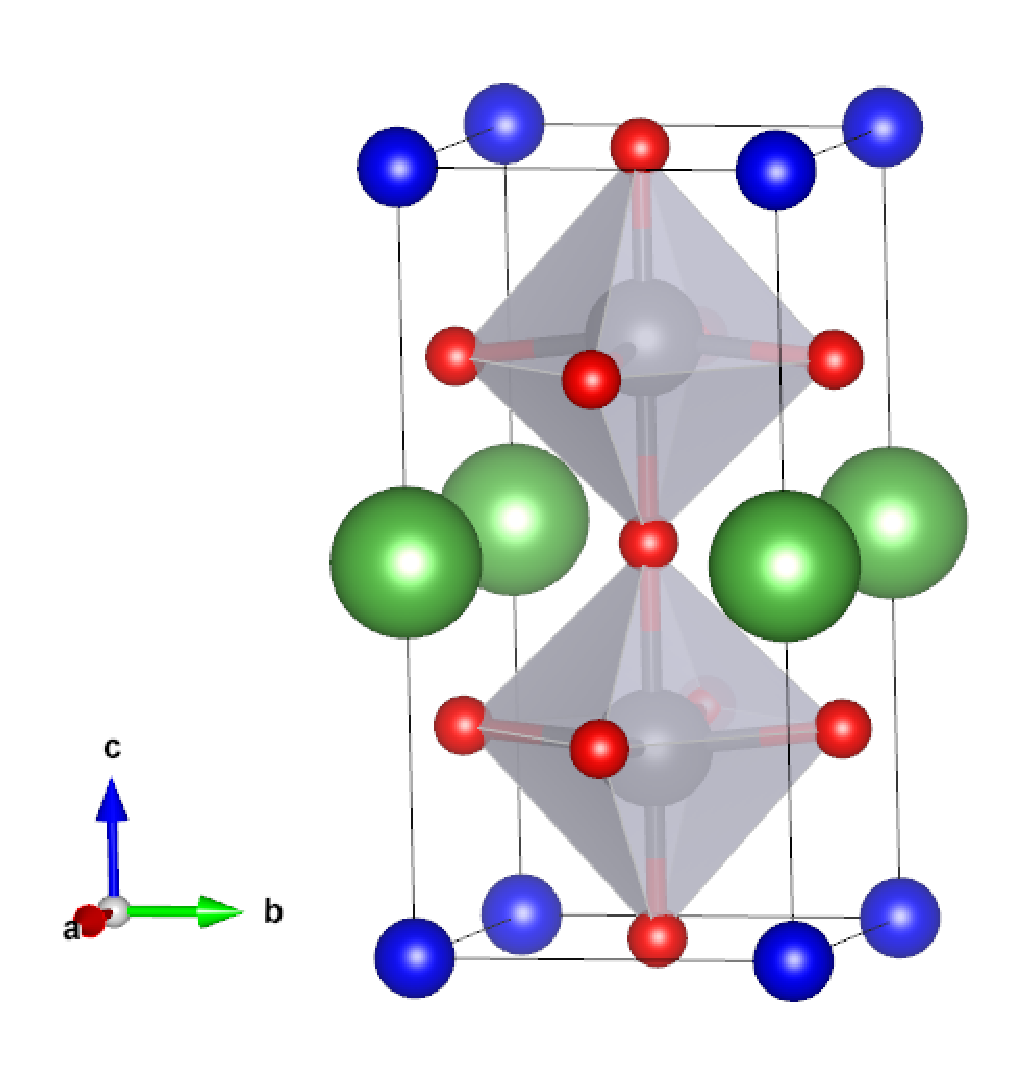
\includegraphics[width=8.6cm]{fig6.eps}
\caption{(color online) 10 atom unit cell of P4/mmm Li$_{0.5}$La$_{0.5}$TiO$_{3}$. Where dark blue spheres are lithium, green spheres are lanthanum, red spheres are oxygen, and grey spheres inside of octahedra are titanium.\label{LLTO_unit_cell}}
\end{figure}
\subsection{Computational Details}
In this work a 3$\times$3$\times$1 90 atom supercell with periodic boundary conditions of the unit cell depicted in Fig. \ref{LLTO_unit_cell} was used as an approximation to bulk Li$_{0.5}$La$_{0.5}$TiO$_{3}$. While not an ideal size as it is  restrictive of the possible lattice configurations and to the types of domains of octahedral tilting that can form it is the largest supercell practical for performing the configurational Monte Carlo in this work. 

An important aspect of completing this study is a scheme for producing the initial and perturbed configurations in the iterative process of the B$_L$ENDER algorithm. The scheme used in this study was to first generate a set of lithium and lanthanum randomly placed on the high symmetry A-sites where occupancy is restricted to one, then a small amount of noise on the order of $\pm$0.2 $\AA$ was added to each lithium and lanthanum coordinate. These configurations were then relaxed to a local minimum which formed the first set of configurations in the iterative process.  Then the perturbed configurations  were formed by swapping a random lithium and lanthanum atom and placing them back on the high symmetry A-site along with a new amount of random noise, these configurations where then relaxed to a local minimum. The random noise off the A-site served to assist searching the distorted lattice configuration space. 

The method used in the calculation of the total energies of the lattice configurations of LLTO in this work was density functional theory using the Vienna \textit{Ab-initio} Simulation Package (VASP) \cite{Vasp1,Vasp2,Vasp3,Vasp4} within the projector augmented wave formalism (PAW)\cite{Blochl}. The Perdew-Burke-Ernzerhof (PBE) variant of generalized gradient approximation was used for the exchange and correlation functional\cite{PBE}. The valence electron configurations for the PAW data sets were; 5p$^{6}$5d$^{1}$6s$^{2}$ for La, 2s$^{1}$ for Li, 3p$^{6}$3d$^{2}$3s$^{2}$ for Ti, and 2s$^{2}$2p$^{4}$ for O. The calculations also took advantage of the ``soft'' option for La and O.   The total energy cut off for expansion of the plane waves was 250 eV.  Self consistent cycles were converged with a energy difference of $<$ 2.5e-5 eV and relaxation  of atomic coordinates was terminated when the difference in total energy between ionic relaxation steps was $<$ 2.5e-4 eV. Electronic occupations used Guassian smearing with a width of 0.05 eV.  A 1$\times$1$\times$2 gamma centered k-point mesh was used for the 3$\times$3$\times$1 supercells of the LiLaTiO6 unit cell. These cutoffs and parameters were chosen to maximize computational efficiency while retaining enough accuracy to capture important physical properties of LLTO.  Each calculation of an energy was completed with a 36 processor broadwell node with an average wall time of 15 minutes per calculation.  To test the accuracy of these methods 10 structures were calculated with fixed coordinates at these convergence criteria and more accurate PAW data sets and cutoffs. The more accurate PAW data sets included the valence electron configurations; 5s$^{2}$5p$^{6}$5d$^{1}$6s$^{2}$ for La, 1s$^2$2s$^{1}$ for Li, 3p$^{6}$3d$^{2}$3s$^{2}$ for Ti, and 2s$^{2}$2p$^{4}$ for O.  The cutoffs for the more accurate calculations were 450 eV for the plane wave basis, and 2$\times$2$\times$3 gamma centered k-points. The average magnitude  in relative energy between structures from this test was 0.05 eV. 

  An important point to make about the calculations in this research is that they  included 0 K static lattice internal energies, did not include phonon free energies, and they did not take into account relaxation of lattice parameters\cite{Holzwarth_group}. Ideally for fixed lattice parameters we would evaluate the parition function\cite{partition}, 
\begin{equation}
Z = \sum_{i=1}^{\Omega} e^{-\frac{(u_i + f_i(T))}{K_bT}}\;.
\label{basicpartition}
\end{equation}
 Where $T$ is the temperature, $k_B$ is Boltzmann's constant, $u_i$ is the static lattice internal energy for configuration $i$, and $f_i(T)$ is the temperature dependant phonon free energy for configuration $i$. A configuration is defined in this work as a local minimum of the Born Oppenheimer potential energy surface. This form of the parition function poses the problem that the density of states is now temperature dependant.  Take $u_i + f_i(T)\equiv e_i(T)$, let $W$ be the number of unique $e_i(T)$, and $F_j(T)$ be the unique $e_i(T)$ then, 
 \begin{equation}
 Z = \sum_{j=1}^{W}G(F_j(T))e^{-\frac{F_j(T)}{k_bT}}\;.
 \end{equation}
 This is a problem because to employ the Monte Carlo methods discussed in this work they would have to be applied at different temperatures which defeats the original purpose. This problem could be addressed by taking $U_j$ to be the unique $u_i$, $\Pi$ to be the number of $U_j$, and then considering a different form of the parition function in Eq. \ref{basicpartition}, 
 \begin{equation}
 Z= \sum_{j=1}^{\Pi}<e^{-\frac{f_i(T)}{k_BT}}>_jG(U_j)e^{-\frac{U_j}{K_bT}}\;.
 \end{equation}
 Here $<\exp(-f_i(T)/k_BT)>_j$ is the arithmetic average of $\exp(-f_i(T)/k_BT)$ over all configurations with static lattice internal energy $U_j$. In this form the static lattice density of states $G(U_j)$ could first be determined with the Monte Carlo methods described in this work and then the $<\exp(-f_i(T)/k_BT)>_j$ could then be approximated by randomly choosing some of the perturbed configurations for each $U_j$ to evaluate the phonon density of states. With the randomly generated phonon densities of states the $<\exp(-f_i(T)/k_BT)>_j$ could be approximated for any temperature. Even in this form though the computational expense is beyond the scope of this work as phonon calculations require high cutoffs and even within the harmonic approximation are much more computationally expense than static lattice calculations\cite{dfpt_phonons}. So in this work the approximation, 
 \begin{equation}
 Z\approx \sum_{j=1}^{\Pi}G(U_j)e^{-\frac{U_j}{K_bT}}\;,
 \end{equation}
 is made. This is reasonable because the phonon free energies are expected to vary much less from configuration to configuration than the static lattice internal energies. A final comment is that relaxation of the lattice paramters could be accomplished by calculating the partition function on a grid of lattice constants, then a free energy surface could be interpolated and the lattice paramaters minimizing the free energy determined as a function of temperature. This procedure is also beyond the scope of the current research. 
 
  The calculations were performed at the experimental lattice parameters 3.8688 $\AA$ for a- and b-axes, and 7.7463 $\AA$ for c-axis. The parameters for the B$_L$ENDER algorithm were $\mathcal{S}=$ 10 and $N=$ 1. The bin width used for determining $G_r(E_j)$ was chosen to be 0.02 eV. The value of $\Omega$ was estimated as 100 times the combinatoric number of configurations of the lithium and lanthanum ordering onto the A-site  given as, 
\begin{equation}
\Omega \approx 100\frac{18!}{9!9!} \;.
\label{omegaguess}
\end{equation}
While an exact value of $\Omega$ is not needed for the algorithm to converge experience from the 2d Ising model suggests that being within several orders of magnitude is sufficient. Estimating that $\Omega$ is greater than the combinatoric calculation of the lithium and lanthanum in the A-site cages comes from the possibility of multiple distinct lattice distortions for each type of A-site cage configurations. An approximate upper bound on the number of distinct lattice distortions for each A-site cage configuration can be based on the experimental and theoretical known that lithium tend to occupy the six possible sites corresponding to local minimum near the oxygen windows connecting different  A-site cages and that lanthanum tend to occupy the center of the cage \cite{Asitedistribution,imaginary_phonons,Li_La_ordering_computational,lithiumpos}. If every lithium could occupy one of these six locations within the A-site cage irrespective of the ordering of the other lithium the number of distinct lattice distortions could be estimated as $6^{9}\approx 1e7$. So the approximation $\Omega  \lessapprox 1e7  \frac{18!}{9!9!}$ can be made. It is physically reasonable that a significant fraction of these configurations will be unstable so that the estimate of $\Omega$ in Eq. \ref{omegaguess} is likely to be within several orders of magnitude of  $\Omega$. 
\subsection{Results}
  Using the parameters and configurational enumeration scheme specified above a simulation was performed to 6,000 iterations for  the 3$\times$3$\times$1,  90 atom supercell. After 150 iterations the algorithm was restricted to look  in the energy range less than 1.25 eV higher than the lowest energy found at that time. This was to improve computational efficiency by preventing the walkers from exploring an unnecessarily high energy range. While 6,000 iterations is not ideally converged, it was sufficient to gain further understanding of the material. In principle it would be desirable to use some type of stopping criteria to determine convergence of the simulation such as in the work of Caprica\cite{halting_wang_and_landau} whom tracked thermodynamic quantities such as the peak of specific heat to determine convergence. In this work convergence is limited by computational resources.   
It is expected that the qualitative aspects of the results are well accounted for despite the limited number of iterations. 
  
The main focus of the results is the nature of the lithium and lanthanum sublattice ordering. To accomplish this the order parameter of interest is that of the occupancy of lanthanum in the lanthanum rich layer along the c-axis.  In the work by Ibarra et al. \cite{P4mmmstrucuture} they refer to this order parameter as $La1$, the same convention will be used in this work. This order parameter, $La1$, is defined as the number of lanthanum in the lanthanum rich layer divided by the total number that could occupy the layer. As an example the unit cell in Fig. \ref{LLTO_unit_cell} would have $La1=1$. It is important to note in this work the 3$\times$3$\times$1 supercell restricts the configurations along the a- and b-axes from having alternate layering of lithium and lanthanum rich layers. Ideally the calculations would be done with at least a 4$\times$4$\times$1 supercell but the computational effort is beyond the scope of this work. The results later will have to be interpreted taking this systematic supercell error into account.  
  
To calculate the ensemble average of these order parameters first arithmetic averages of the order parameter at each energy level $E_j$ are calculated from the perturbed configurations  that occurred during the simulation. The arithmetic average of a general order parameter $O$ over all configurations with energy $E_j$ is denoted by $< O >_j$. Then with these the ensemble average is computed as, 
  \begin{equation}
  \langle O \rangle  =  \sum_{j=1}^{\Pi}< O >_j G_r(E_j) \frac{e^{-\frac{E_j}{k_BT}}}{Z} \;.
  \label{ensembleaverage}
  \end{equation}
  Where $Z= \sum_{j=1}^{\Pi} G_r(E_j) exp(-\frac{E_j}{k_BT})$. 
It is noted that normalization of the relative density of states to the appropriate number of configurations is not necessary for the calculation of the ensemble average of an order parameter. If wanting to compare free energies($-k_BT\ln(Z)$) between phases it would be necessary to normalize the density of states properly to obtain an accurate calculation of the free energy. 

\begin{figure}[h!]
(a)\\
\includegraphics[width=8.6cm]{fig7a.eps}
\centerline{(b)}\\
\includegraphics[width=8.6cm]{fig7b.eps}
\centerline{(c)}\\
\includegraphics[width=8.6cm]{fig7c.eps}
\caption{Plots of $G_r(U_j)$ at (a) 500 iterations, (b) 2,000 iterations, and (c) 6,000 iterations. The plots are normalized by dividing through by the minimum value of $G_r(U_j)$ at that particular iteration. The plots are shown with a log scale on the y-axis.  \label{converge_GE}}
\end{figure}

The first main result is a view of the convergence of $G_r(U_j)$ as a function of the iterations. Here we have switched to using $U_j$ to highlight that the calculations only include 0 K static lattice internal energies as discussed before. In Fig. \ref{converge_GE},  $G_r(U_j)$ is shown at  $I= $ 500, 2000, and 6,000 with the y-axis plotted on a log scale. The  $G_r(U_j)$ shown in Fig. \ref{converge_GE}  are plotted such that the lowest energy of $G_r(U_j)$ found at the particular iteration shown is set to zero, the sharp cutoff at higher energy was the upper limit to energy range, and the plots are normalized by dividing through by the minimum of $G_r(U_j)$ at that iteration.  The main characteristic of the results by 6,000 iterations is the presence of some low energy states seperated by gaps followed by a peak in the density of states at ~0.25 eV followed by a small dip leading to a continous spectrum at higher energy. It is noted, as the iterations increase, that $G_r(U_j)$ for the spectrum of higher energy states becomes noticeably smoother.  The lowest energy configuration is  characterized as having  $La1=1$, that being having alternate layers of lithium and lanthanum along the c-axis. It is not however equivalent to the unit cell shown in Fig. \ref{LLTO_unit_cell}, in that the structure has distinct lattice distortions. 


The next result is the arithmetic averages of the $La1$  order parameter, which are  shown in Fig. \ref{arithemetic_avg}(a) along with the number of samples used to determine each value in Fig. \ref{arithemetic_avg}(b). The results in Fig. \ref{arithemetic_avg}(a) show an overall tendency for more mixing of lithium and lanthanum between layers for higher energies. The ensemble average of $La1$ is shown in Fig. \ref{ensembleOP}, which shows a phase transition from completely segregated lithium and lanthanum between layers to mostly mixed between layers and increased mixing with increasing temperature. In Fig. \ref{ensembleOP} the values for $La1$ range from approximately 0.73 at 650 K to 0.69 at 1500 K.  For the 3$\times$3$\times$1 model the minimum possible value of $La1$ is $5/9 = 0.56$. These results are in qualitative agreement with the $La1=0.53$ reported by Ibarra et al. \cite{P4mmmstrucuture}  and it is expected that that larger supercell models would increase the available configurational entropy and result in a reduced value of $La1$ in the disordered phase. A movie of the convergence of the ensembles average of $La1$ is provided in the supplemental materials, it shows that although the qualitative features of the order parameter remain relatively unchanges starting at $I\approx 600$. 

\begin{figure}[h!]
(a)\\
\includegraphics[width=8.6cm]{fig8a.eps}\\
\centerline{(b)}
\includegraphics[width=8.6cm]{fig8b.eps}
\caption{(a) Arithmetic averages of the $La1$ order parameter as a function of energy. The error bars in (a) are the standard deviation of the mean.  (b) Number of counts to determine each value of the $La1$ order parameter for each energy. For the bins with total count of 1 in (b) the standard deviation of the mean plotted in (a) is simply plotted as zero.  \label{arithemetic_avg}}
\end{figure}

\begin{figure}[h!]
\includegraphics[width=8.6cm]{fig9.eps}
\caption{Ensemble average of the $La1$ order parameter calculated with Eq. \ref{ensembleaverage} as function of temperature. \label{ensembleOP}}
\end{figure}

Some indication of convergence of the 6,000 iterations comes from inspecting the flatness of the histogram $H(U_j)$ of visited energies during the simulation. Why is is in an indicator of convergence can be understood by Eq \ref{adiabatic_distribution} which indicates that the adiabatic distribution of $\mathcal{H}^I$ is flat for bins that converged realtive to each other. If $\mathcal{H}^I$ is flat then the total histogram $H(U_i)=\sum_i=0^I\mathcal{H}^i$ should form a flat histogram.   A histogram of the visited energies during the simulation is shown in Fig. \ref{Htot}. The results show that  the histogram is qualitatively flat for $\gtrapprox $ 0.4 eV. This result along with the counts for calculating the $La1$ order parameter shown in Fig. \ref{arithemetic_avg}(b) suggest that the results are most well converged for $\gtrapprox $ 0.4 eV. In this sense the statement can be made that the strongest result of this computation is the trend for more mixed configurations to have higher energy seen in the range $\gtrapprox $ 0.4 eV. The results below 0.4 eV still provide useful information on the nature of low energy structures.  While the first principles methods used can be considered coarse grained in terms of PAW data sets, total energy cutoffs, and k-points as observed from testing with more accurate methods, the trend seen in figure Fig. \ref{arithemetic_avg}(a) spans an energy range much greater than the expected relative error in energies between structures. It must be said that the ensemble average of $La1$ is highly dependent on the low energy structures as per the exponential nature of the partition function. In this regard the observed phase transition in Fig. \ref{ensembleOP} can not be expected to be an accurate prediction of a transition temperature. The most important result of Fig. \ref{ensembleOP} is the high temperature region above the phase transition showing a tendency for greater mixing of lithium and lanthanum for increasing temperature. 

To gain some further insight into the structures found during the simulation the  lowest energy structure and lowest energy structure with $La1$ != 1 are  shown in  Fig. \ref{lowen_structures}(a) and (b). In Fig. \ref{lowen_structures}(a) it is seen that the lowest energy structure has the lithium and lanthanum completely segregated between layers along the c-axis. In Fig. \ref{lowen_structures}(b)  the  lowest energy structure with $La1$ != 1  has a fully occupied layer of lithium along the a-axis along with two partially occupied layers, this structure is 0.24 eV in energy above the lowest energy structure. Structures similar to that in Fig. \ref{lowen_structures}(b) are in part responsible for the dip in the $La1$ order parameter in Fig. \ref{arithemetic_avg}(a) in the energy range 0.24  to 0.4 eV.  Due to the pseudo cubic nature of the system it is expected that there would be nearly energetically identical structures  consisting of completely segregated lithium and lanthanum layers along the a and b axes. This feature of ambiguity of the orientation of how the lithium and lanthanum rich layers can form  are a likely driving force for the numerous domain boundaries observed in experiments for other stoichiometries synthesized by annealing from high temperature\cite{imaginary_phonons,domainboundaries}. Due to the 3$\times$3$\times$1 supercell used in this study these structures were not possible to realize in the simulation but as evidenced by Fig. \ref{lowen_structures}(b) segragation of the lithium and lanthanum into separate layers is still energetically favorable. A common feature of both Fig. \ref{lowen_structures}(a) and (b) is the lithium sitting off of the high symmetry A-site near the oxygen windows separating A-site cages. This feature has been previously reported experimentally and theoretically in the literature\cite{Asitedistribution,imaginary_phonons,Li_La_ordering_computational,lithiumpos}. 
\\


\begin{figure}
(a)\\
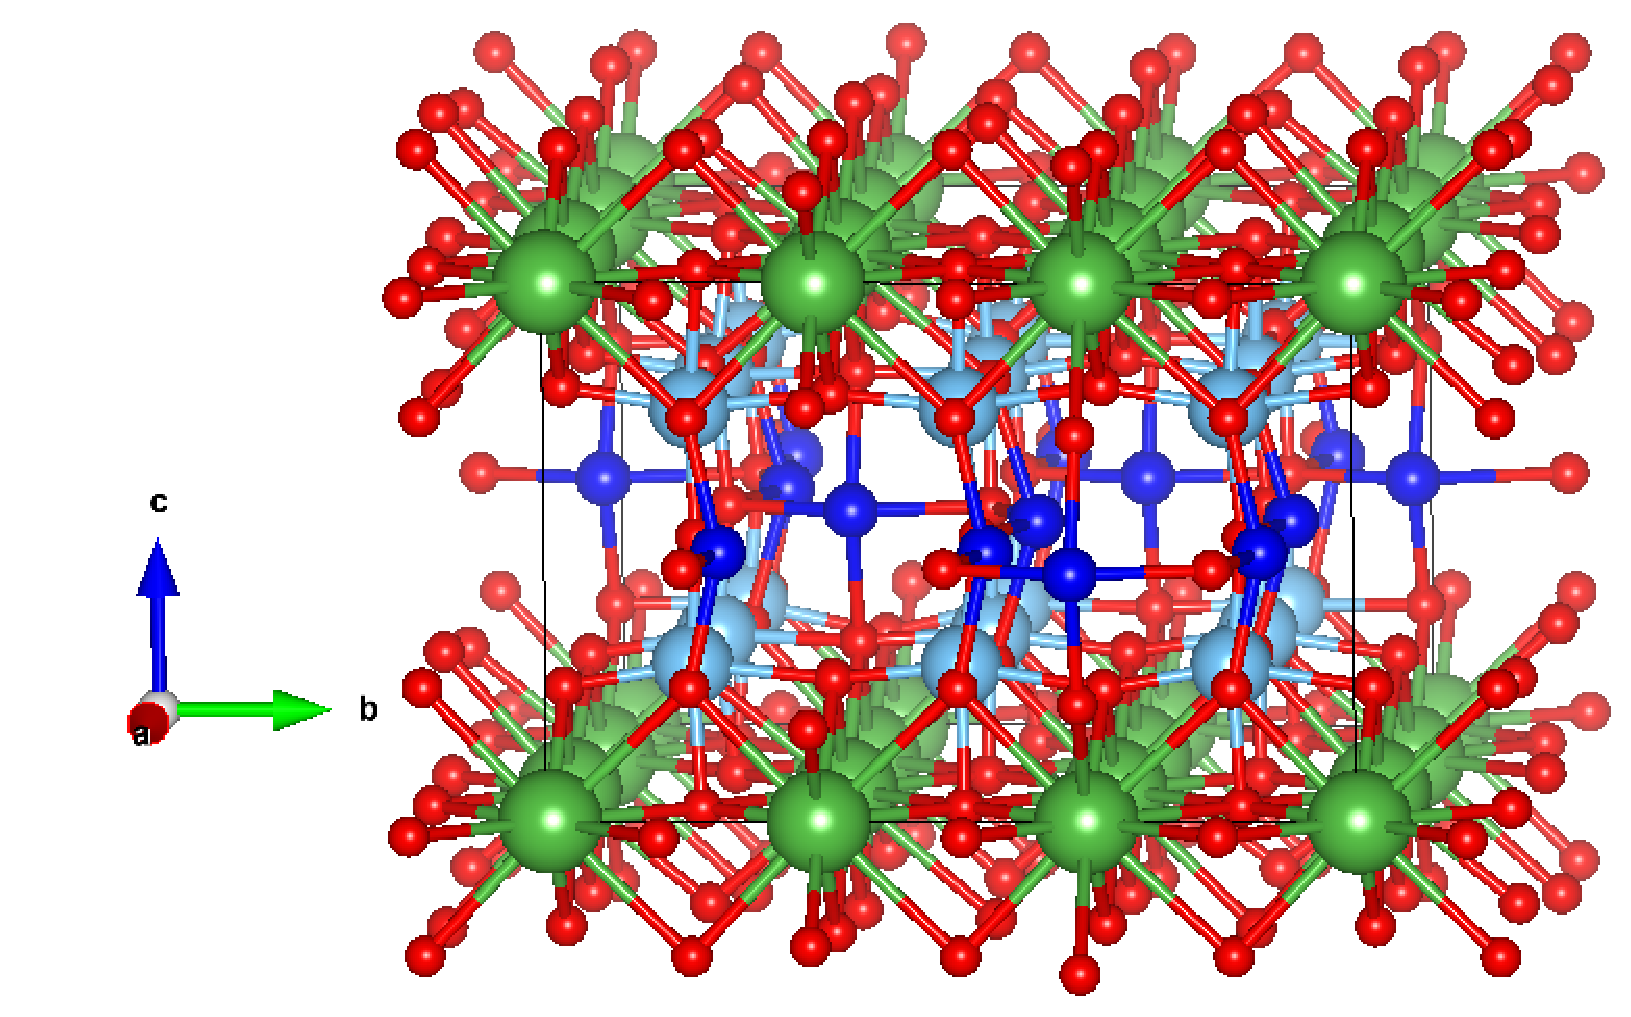
\includegraphics[width=8.6cm]{fig10a.eps}\\
(b)\\
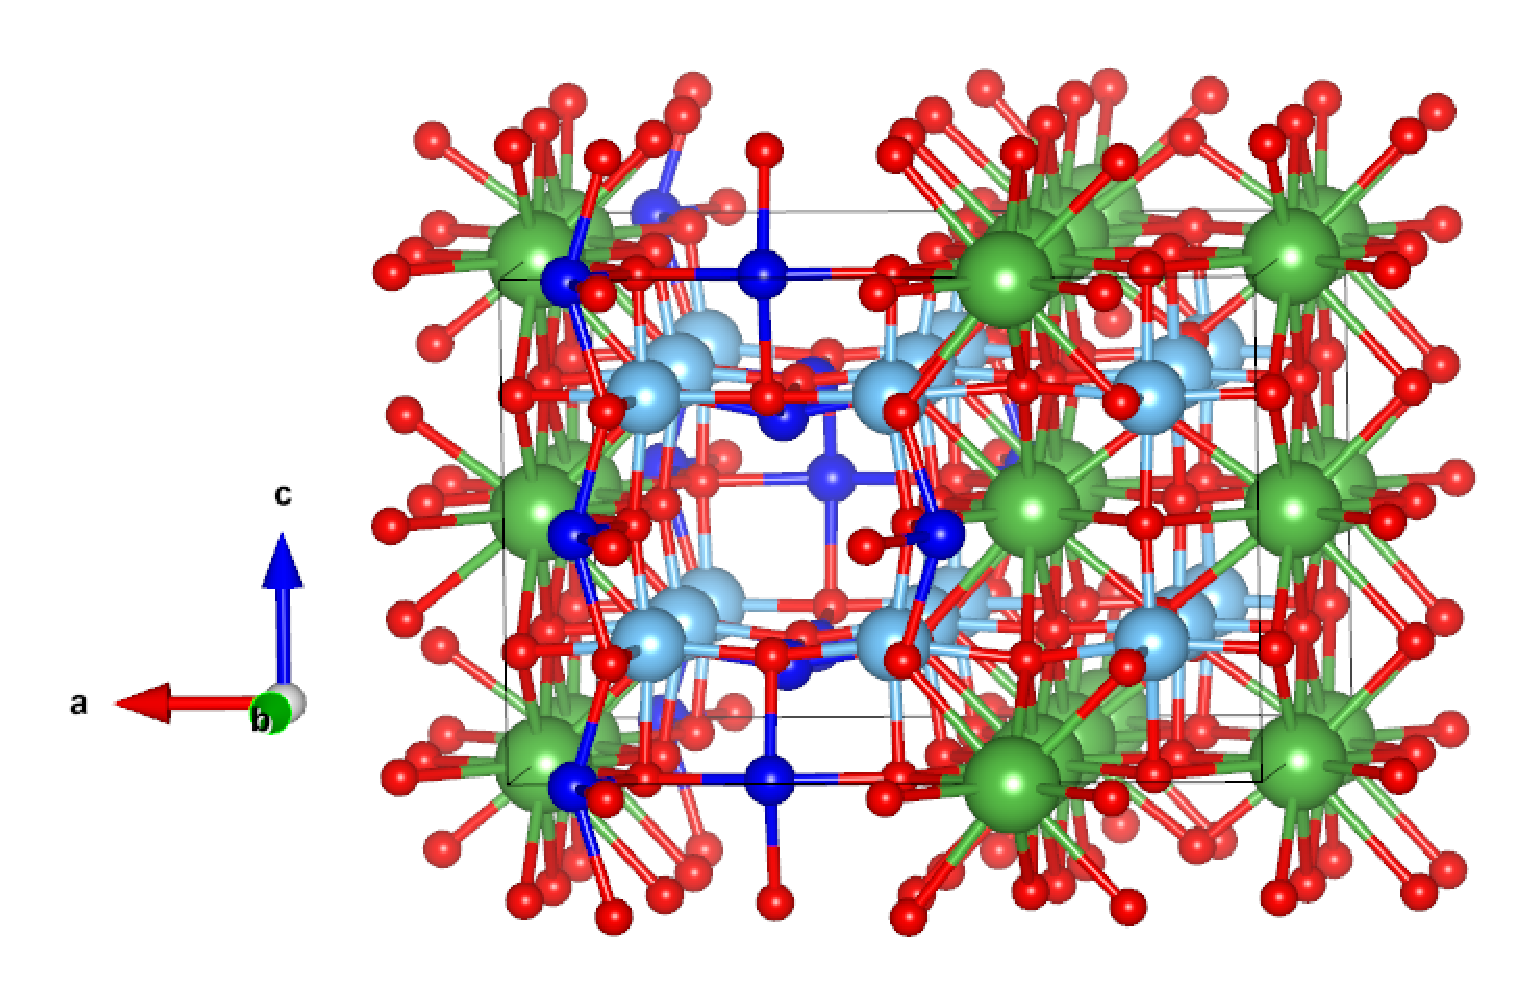
\includegraphics[width=8.6cm]{fig10b.eps}
\caption{(color online) (a) Lowest energy structure found during simulation. (b)  Lowest energy structure found during the simulation that has $La1$  $!= 1$. Where dark blue spheres are lithium, green spheres are lanthanum, red spheres are oxygen, and light blue spheres  are titanium. \label{lowen_structures}}
\end{figure}

\begin{figure}
\includegraphics[width=8.6cm]{fig11.eps}
\caption{Plot of the histogram of the visited energies over the 6,000 iterations of the simulation. Visited here means the accepted energies as per step 3 of Eq. \ref{blender}.\label{Htot}}
\end{figure}

\section{Conclusions}
\label{sec5}
 This work has presented a parallel variant of the Wang and Landau algorithm referred to as B$_L$ENDER( B$_L$end Each New Density Each Round). The algorithm was developed purposely for use with disordered crystal sublattices and is naturally parallel. It's design makes it facile to implement on a mid level high performance computer such as Argonne's BEBOP where jobs for a structural energy calculation can be independently submitted to compute nodes  and managed by a script running on a head node. It was trialed using the 2d Ising model and showed good performance for the 10$\times$10 Ising model with a minimal number of implementation parameters. Results for the 32$\times$32 Ising model suggest the algorithm could have applicability to larger system sizes provided a tuning parameter is chosen appropriately to maximize performance, currently it is not known how to choose this parameter before hand without numerical testing. Comparing performance with the the original Wang and Landau algorithm showed that while B$_L$ENDER tends to decrease in error over the simulation while the error in the original Wang and Landau rises to a peak early in the simulation and then drops suddenly. Long time performance of the B$_L$ENDER algorithm and the original Wang and Landau algorithm was found to be comparable.  In the case of using one walker the B$_L$ENDER algorithm was also found to have similar behavior as to the N-fold 1/t algorithm of Belardinelli et al.\cite{saturation}. Convergence of the algorithm is established within an adiabatic assumption and this analysis was abale to correctly derive the time dependence of the modification factor for the algorithm for the 8$\times$8 Ising model.  Knowledge gained from testing with the 2d Ising model allowed for an informed implementation to the real material science problem of studying the lithium and lanthanum sublattice disorder of Li$_{0.5}$La$_{0.5}$TiO$_{3}$ using density functional theory methods. The simulations of the disordered lithium ion conductor LLTO were in qualitative agreement with experiment and provided further insight into the disordered nature of the material. It was found that lower energy structures favored segregating lithium and lanthanum into separate layers and that structures with lithium and lanthanum mixed between layers were on average higher in energy than more segregated structures. Thermodynamic analysis of the order parameter related to lithium and lanthanum intermixing between layers showed a phase transition between completely segregated  to mostly mixed tending to more mixed at higher temperatures. Overall the results show that the algorithm performed well in simulating both the 2d Ising model and with first principles calculations of a real material system. 

\begin{acknowledgments}
This work was supported by the Center for Electrical Energy Storage: Tailored Interfaces, an Energy Frontier Research Center funded 
by the US Department of Energy, Office of Science, Office of Basic Energy Sciences at Argonne National Laboratory under Contract DE-AC02-06CH11357.
I would like to thank the Laboratory Computing Resource Center (LCRC) faculty of Argonne National Lab for their support and maintenance of the computing resources that made this project possible. 
\end{acknowledgments}

\bibliography{Manuscript}
\bibliographystyle{apsrev4-1}

\end{document}
